\ChapterAuthor[%
Structure Commands]{%
Structure Commands}{%
Roger \Name{Rousseau}\and Christian \Name{Scheen}}
\label{chap-struct}

This chapter describes the main commands that structure the whole book
(\latex{} preamble, front matter, main matter, and back matter; these great
subdivisions may then contain parts, chapters, sections, paragraphs, and
smaller components).

\section{Books, monographs, and edited collections}
\label{type-ouvrage}
\index{book (definition)}
\index{monograph (definition)}
\index{edited collection (definition)}

In accordance with the \Hermes{} terminology, let us use the term \emph{book}
for any typeset document whose general layout is based on the notion of a
chapter made up of several pages.
Chapters may be gathered within larger parts, and they are subdivided with
the help of smaller subtitles characterized by their level~$n$.
Subtitles of level~$1$ down to level~$4$ are allowed; in \latex{}, these
correspond respectively to \cmd{section} (level~$1$), \cmd{subsection}
(level~$2$), \cmd{subsubsection} (level~$3$), and \cmd{paragraph} (level~$4$)
commands.
According to the \hermes{} guidelines, level~$n \geq 5$ subtitles must not
appear in any actual book; in \latex{} parlance, this means that authors
should not use the \cmd{subparagraph} (level~$5$) command (see
Table~\ref{tab:Subtitles}).
Monographs, edited collections, joint works, technical reports, handbooks,
and doctoral dissertations may all be considered as books from the structural
point of view.
\Hermes{} defines monographs and edited collections; let us specify this
terminology.

\NumberedDefinition{%
In a \emph{monograph}, all chapters are written by the same author or by the
same group of authors.\index{monograph (definition)}
The book possesses a single bibliography chapter whose contents is therefore
shared by all regular chapters; the bibliography is typeset at the end of the
book, before the index.}

\NumberedDefinition{%
In an \emph{edited collection}, each chapter is written by its own author or
by its own group of authors.\index{edited collection (definition)}
The book is coordinated by one or more scientific directors.
Each chapter possesses its specific bibliography section; the bibliography is
typeset at the end of the chapter.}

\begin{Table}[!htbp]{%
\latex{}'s standard sectioning commands\\
(\latex{} levels coincide with \hermes{} levels)\label{tab:Subtitles}}
\setlength{\tabcolsep}{4pt}
\renewcommand{\arraystretch}{1.2}
\begin{tabular}{|l|r|l|}
 \hline
 \multicolumn{1}{|c|}{\textbf{Command}}
 & \multicolumn{1}{c|}{\textbf{Level}}
 & \multicolumn{1}{c|}{\textbf{Automatic style}} \\ \hline
 \cmd{part}\index{part@\cmd{part}}
 & $-1$ & flush right on a special page \\
 \cmd{chapter}\index{chapter@\cmd{chapter}}
 & $0$ & flush right or centered${}^{\dagger}$ \\
 \cmd{section}\index{section@\cmd{section}}
 & $1$ & upright shape, bold series \\
 \cmd{subsection}\index{subsection@\cmd{subsection}}
 & $2$ & italic shape, bold series \\
 \cmd{subsubsection}\index{subsubsection@\cmd{subsubsection}}
 & $3$ & italic shape, medium series \\
 \cmd{paragraph}\index{paragraph@\cmd{paragraph}}
 & $4$ & upright shape, medium series \\
 \cmd{subparagraph}\index{subparagraph@\cmd{subparagraph}}
 & $5$ & forbidden in \hermes{} books \\ \hline
 \multicolumn{3}{@{}l}{$\dagger$~Flush right for monographs, centered for
 edited collections.}
\end{tabular}
\end{Table}

All books are laid out along three great subdivisions:
\begin{enumerate}
 \item\index{frontmatter@\cmd{frontmatter}}
 the \emph{front matter} (\cmd{frontmatter}) contains the title page, the
 table of contents, and small unnumbered chapters.
 These unnumbered chapters have usually no subtitles at all; therefore, one
 may include, for instance, a preface, a foreword, and a small introduction
 in the front matter;
 \item\index{mainmatter@\cmd{mainmatter}}
 the \emph{main matter} (\cmd{mainmatter}) contains all regular numbered
 chapters.
 Optionally, those regular chapters may be followed by numbered appendices;
 \item\index{backmatter@\cmd{backmatter}}
 the \emph{back matter} (\cmd{backmatter}) contains the bibliography chapter
 (only in the case of a monograph), an optional glossary, and the index.
 These are all unnumbered chapters.
\end{enumerate}

Chapter numbering (and appendix numbering) is automatic and depends on its
position amongst these subdivisions.
For instance, a small introduction with few subtitles shall be placed in the
front matter, where it will automatically be typeset as an unnumbered
chapter.
On the other hand, a longer and/or structured introduction shall be placed at
the beginning of the main matter, where it will automatically be typeset as
a regular numbered chapter (of course, its subtitles will automatically be
numbered, too).
In order to disable the appearance of an unnumbered chapter in the table of
contents, one can use the starred form of the \cmd{chapter} command (namely,
\cmd{chapter*\{\meta{Chapter Title}\}}).\index{chapter*@\cmd{chapter*}}

Commands that define the general layout of the book shall be gathered in the
master \latex{} source file that we describe below.

\section{The master \latex{} source file}
\index{master latex source file@master \latex{} source file}

The master \latex{} source file defines the general layout of the book and
consists of two parts: the preamble (between the \cmd{documentclass} and the
\cmd{begin\{document\}} commands) and the document body (between the
\cmd{begin\{document\}} and the \cmd{end\{document\}} commands).
See Figure~\ref{prelude} for details.

\begin{Figure}[!htbp]{%
General structure of the \latex{} preamble\label{prelude}}
\begin{fminipage}
\begin{verbatim}

 \documentclass[<class options>]{ouvrage-hermes}[2005/11/14]

 % The LaTeX preamble may contain package loading commands and
 % user-defined LaTeX commands and environments.  The optional
 % \usepackage, \newcommand, and \newenvironment commands shall
 % be included here.

 \title[%
 Shortened Book Title]{%
 Complete Book Title\\
 with Optional Line Breaks}

 \author{%
 John \Name{Smith}\\ Paul \Name{Jones}}

 \date{%
 November~14, 2005}

 \makeindex

 \begin{document}
 % The document body is described in another section.
 \end{document}

\end{verbatim}
\end{fminipage}
\index{documentclass@\cmd{documentclass}}
\index{usepackage@\cmd{usepackage}}
\index{newcommand@\cmd{newcommand}}
\index{newenvironment@\cmd{newenvironment}}
\index{title@\cmd{title}}
\index{author@\cmd{author}}
\index{date@\cmd{date}}
\index{makeindex@\cmd{makeindex}}
\index{begindocument@\cmd{begin\{document\}}}
\index{enddocument@\cmd{end\{document\}}}
\index{document@\env{document}}
\end{Figure}

The \cmd{documentclass} command is given the \verb+ouvrage-hermes+ mandatory
parameter that specifies the name of the \class{ouvrage-hermes} document
class, and the \meta{class options} optional parameter that controls various
specific aspects of document typesetting; available class options are
described below.

\section{Class options}
\index{class option}

The default behavior of the \class{ouvrage-hermes} document class makes it
possible to typeset a monograph written in French, without crop marks, and
without blank pages printing.
According to the desired book type, the following class options will be used
(see also Table~\ref{tab:ClassOptions}):
\begin{itemize}
 \item\index{treatise class option@\texttt{treatise} (class option)}
 the \verb+treatise+ class option typesets an edited collection.
 The default behavior is to typeset a monograph;
 \item\index{english class option@\texttt{english} (class option)}
 the \verb+english+ class option typesets a book written in English.
 The default behavior is to typeset a book written in French.
 Obviously, the \latex{} format must include word-breaking hyphenation
 patterns for the intended language\footnote{The \latex{} format generation
 process is beyond the scope of this user's guide.
 Let us stress that \hermes{} uses French and American English hyphenation
 patterns.}.
 This class option defines the basic language of the book.
 However, if specific chapters are not written in the basic language, these
 shall start with the \cmd{selectlanguage\{\meta{language}\}} language
 selection command;\index{selectlanguage@\cmd{selectlanguage}}
 \item\index{cropmarks class option@\texttt{cropmarks} (class option)}
 the \verb+cropmarks+ class option draws the page borders: a first rectangle
 corresponds to the text dimensions, and a taller one shows the page limits
 (after the trimming process).\label{opt-cropmarks}
 The default behavior is to disable crop marks.
 The final copy of a book shall not exhibit crop marks;
 \item\index{allpages class option@\texttt{allpages} (class option)}
 the \verb+allpages+ class option prints out blank pages.
 The default behavior is to suppress blank pages printing.
 This class option enables one to save printing (let us recall that chapters
 always start on odd pages).
 The final copy of a book shall enable blank pages printing.
\end{itemize}

\begin{Table}[!htbp]{%
Class options and their implied behavior\label{tab:ClassOptions}}
\setlength{\tabcolsep}{4pt}
\renewcommand{\arraystretch}{1.2}
\begin{tabular}{|l|l|l|}
 \hline
 \multicolumn{1}{|c|}{\textbf{Class option}}
 & \multicolumn{1}{c|}{\textbf{Implied behavior}}
 & \multicolumn{1}{c|}{\textbf{Default behavior}} \\ \hline
 \texttt{treatise}
 \index{treatise class option@\texttt{treatise} (class option)}
 & typeset an edited collection & typeset a monograph \\
 \texttt{english}
 \index{english class option@\texttt{english} (class option)}
 & typeset a book in English & typeset a book in French \\
 \texttt{cropmarks}
 \index{cropmarks class option@\texttt{cropmarks} (class option)}
 & enable crop marks drawing & disable crop marks drawing${}^{\dagger}$ \\
 \texttt{allpages}
 \index{allpages class option@\texttt{allpages} (class option)}
 & enable blank pages printing${}^{\dagger}$ & disable blank pages printing
 \\ \hline
 \multicolumn{3}{@{}l}{$\dagger$~Required behavior for the final copy.}
\end{tabular}
\end{Table}

Let us now consider the \latex{} preamble details.

\section{\latex{} preamble}
\index{preamble}
\index{latex preamble@\latex{} preamble}

The \latex{} preamble shall successively contain (see Figure~\ref{prelude}):
\begin{enumerate}
 \item\index{usepackage@\cmd{usepackage}}
 optional package loading commands.
 For instance, one might want to use the \cmd{usepackage[fleqn]\{amsmath\}}
 command in order to load advanced mathematical structures designed by the
 American Mathematical Society;
 \item\index{newcommand@\cmd{newcommand}}
 \index{newenvironment@\cmd{newenvironment}}
 \index{def@\cmd{def}}
 optional user-defined commands and environments.
 User-defined structures shall be defined with the \cmd{newcommand} and
 \cmd{newenvironment} \latex{} commands; one should not use plain \tex{}
 commands (such as \cmd{def},~etc.\@);
 \item\index{title@\cmd{title}}
 the \cmd{title[\meta{Shortened Book Title}]\{\meta{Complete Book Title}\}}
 statement.
 The \meta{Shortened Book Title} parameter is used as the running title on
 even pages and its length shall not exceed~55\,mm in 9\,pt~font size; the
 \class{ouvrage-hermes} document class raises a warning message when this
 condition is not met;
 \item\index{author@\cmd{author}}\index{Name@\cmd{Name}}
 the \cmd{author} statement.\index{backslashbackslash@\bsbs{}}
 The \cmd{Name} command distinguishes surnames from given names.
 The \bsbs{} command separates the full names of successive authors.
 The example below shows the exact syntax;
 \item\index{date@\cmd{date}}
 the \cmd{date\{\meta{version date}\}} statement, as usual.
\end{enumerate}

\Example{%
The \cmd{author} statement shall be given as follows:}
\begin{quote}
\begin{verbatim}
\author{%
<Given name #1> \Name{<Surname #1>}\\
<Given name #2> \Name{<Surname #2>}}
\end{verbatim}
\end{quote}

\section{Document body}
\index{document body}

Within the document body, the top-level structure commands are
\cmd{frontmatter},\index{frontmatter@\cmd{frontmatter}}
\cmd{mainmatter},\index{mainmatter@\cmd{mainmatter}} and
\cmd{backmatter}.\index{backmatter@\cmd{backmatter}}

The contents of each chapter shall be placed within one single dedicated
file; chapter files shall be included with the\index{include@\cmd{include}}
\cmd{include} (not\index{input@\cmd{input}} \cmd{input}) command in the
master \latex{} source file.
In the case of an edited collection, where each chapter has its own
bibliography section, this requirement is mandatory.

Some unnumbered chapters such as the table of contents, the bibliography
chapter (in the case of a monograph), and the index are produced by specific
commands placed at appropriate positions in the master \latex{} source file.

The optional \cmd{appendix}\index{appendix@\cmd{appendix}} command notifies
the start of the appendices.
In order to generate appropriate table of contents entries, the
\cmd{appendix}\index{appendix@\cmd{appendix}} command shall be placed at the
beginning of the first included appendix file (not in the master \latex{}
source file itself).

Figure~\ref{corps-docu} gives a rather complete example of document body;
see Figure~\ref{prelude} for its location within the whole master \latex{}
source file.

As already mentioned, authors should definitely \emph{not} use the \latex{}
source files of this user's guide as the starting point of the \latex{}
source files of any actual book; the \dir{Ouvrage-Hermes} top-level directory
holds suitable templates of master \latex{} source files:
\begin{itemize}
 \item\index{hsp-monograph.ltx@\file{hsp-monograph.ltx}}
 for monographs, use the \file{hsp-monograph.ltx} template,
 \item\index{hsp-treatise.ltx@\file{hsp-treatise.ltx}}
 for edited collections, use the \file{hsp-treatise.ltx} template.
\end{itemize}

\begin{Figure}[!htbp]{%
General structure of the document body\label{corps-docu}}
\begin{fminipage}
\begin{verbatim}

 \begin{document}

 \frontmatter %--------------------

 \maketitle
 \include{preface}
 \tableofcontents
 \chapter*{Foreword}
\addtocontents{toc}{\protect\contentsline{chapter}{Foreword}{\thepage}}
\addtocontents{toc}{\protect\TextInToc{0}{0pt}{%
 Roger \Name{Rousseau}, Christian \Name{Scheen}}}
\addtocontents{toc}{\protect\addvspace{5pt plus 1pt minus 1pt}}

The aim of this document is to describe how to use \latex{} in order to
typeset books (namely, monographs or edited collections; this terminology
will be defined later on in this document) according to the
\Hermes{}~(\HSP{}) guidelines and instructions to authors.
The \oh{} package contains a \latex{} document class file, a \bibtex{}
alphanumeric bibliography style file, and a \mkndx{} index style file.
Index typesetting is made easier through a basic Bourne shell script and two
associated \awk{} (or \gawk{}) filters.
Of course, the use of this indexing mechanism is completely optional;
everything is possible (but sometimes more involved) through the standard
\mkndx{} program that comes with every \tex{} system distribution.
Finally, the \oh{} package contains a \Makefile{} script for the \make{}
utility; its use is also optional and makes it easy to keep the main target
(namely, the final document in PostScript format) current, based on
differences in the modification times of the \tex{} source files that the
PostScript target is dependent on.

Let us stress that users of the \oh{} package should definitely \emph{not}
use the \latex{} source files of this user's guide as the starting point of
the \latex{} source files of any actual book (this user's guide is a very
special case that is laid out as an edited collection, but that also
possesses some monograph features).
The \oh{} package provides users with appropriate templates instead; see the
\file{hsp-monograph.ltx} and \file{hsp-treatise.ltx} files in the
\dir{Ouvrage-Hermes} top-level directory for details.

\latex{} itself is Leslie Lamport's generic typesetting system~\cite{Lam94}
that uses Donald E.\@~Knuth's \tex{} formatting system~\cite{Knu86} as its
underlying engine.
The main idea behind \latex{} is to let the user concentrate on the layout
and the structure of the document rather than on formatting details.
With this aim in mind, the \latex{} system adds an abstraction layer onto the
plain \tex{} commands; the user is provided with high-level commands that
make document typesetting easier.
The \latex{} format contains a precompiled image of all these \latex{}
commands, the \tex{} font metrics~(``.tfm'') information for preloaded fonts,
and a set of word-breaking hyphenation patterns for each language that one
might want to use.
A number of excellent books on \latex{} and related tools and techniques are
available.
In addition to the books by Knuth~\cite{Knu86} and Lamport~\cite{Lam94}, let
us refer to the introduction guide by \hbox{Helmut} Kopka and Patrick
W.\@~Daly~\cite{KD04}, to the editions of the \latex{} ``companion'' by Frank
Mittelbach \emph{et~al.\@}~\cite{GMS94, MGBCRDS04}, to the \latex{} graphics
``companion'' by Michel Goossens \emph{et~al.\@}~\cite{GRM97}, and to the
\latex{} Web ``companion'' by Michel Goossens \emph{et~al.\@}~\cite{GRGMS99}.
French-speaking users are moreover referred to the introduction guides by
Christian Rolland~\cite{Rol99} and Bernard Desgraupes~\cite{Des03}.

\section*{Typographic conventions}
\addtocontents{toc}{\protect\contentsline{section}{%
 Typographic conventions}{\thepage}}
\index{typographic convention}

We use the standard typographic conventions throughout the document (see for
instance~\cite[p.\@~\hbox{11-13}]{MGBCRDS04}):
\begin{itemize}
 \item programs (such as \mkndx{}, \xindy{}, \make{}, \awk{}, and \gawk{})
 and drivers (such as \dvips{} and \pstopdf{}) are typeset in sans serif text
 font;
 \item scripts (such as \Makefile{} and \Makeindex{}) and so-called filters
 (such as \preawk{} and \postawk{}) are typeset in monospaced typewriter text
 font;
 \item \LaTeX{}, \bibtex{}, and \mkndx{} classes and style files (such as
 \class{book}, \style{chapterbib}, \bstyle{ouvrage-hermes}, and
 \istyle{ouvrage-hermes}) are typeset in sans serif text font;
 \item \LaTeX{} commands and environments (such as \cmd{makeindex} and
 \env{flushright}) are typeset in monospaced typewriter text font.
 Besides, environments are typeset in slanted shape font;
 \item place-holders (also known as meta-variables) are typeset in italic
 shape font between ``$\langle$''~and~``$\rangle$'' angle brackets (for
 instance, \meta{text}).
\end{itemize}


\vspace{11pt}

\begin{flushright}
 Roger \Name{Rousseau}\\
 Christian \Name{Scheen}
\end{flushright}

%%% Local Variables: 
%%% mode: latex
%%% TeX-master: "users-guide.ltx"
%%% End: 

 \PresentationOfAuthors{Introduction written by~}
\ChapterAuthor[%
Introduction]{%
Introduction}{%
Roger \Name{Rousseau}\and Christian \Name{Scheen}}
\label{chap-introduction}

This document describes how to use \latex{} in order to typeset books
(namely, monographs or edited collections) according to the
\Hermes{}~(\HSP{}) guidelines and instructions to authors, with the \oh{}
package.
Many examples are given (\latex{} source files templates, syntax of user
commands and environments,~etc.\@).

The \oh{} package consists of the following files:
\begin{itemize}
 \item\index{ouvrage-hermes.cls@\class{ouvrage-hermes}}
 the \class{ouvrage-hermes} \latex{} document class file.
 It shall be used instead of the \class{book} standard \latex{} document
 class file;
 \item\index{ouvrage-hermes.bst@\bstyle{ouvrage-hermes}}
 the \bstyle{ouvrage-hermes} \bibtex{} bibliography style file.
 It shall drive the \bibtex{} program in order to produce appropriate
 alphanumeric bibliographies;
 \item\index{ouvrage-hermes.ist@\istyle{ouvrage-hermes}}
 the \Makeindex{}\index{Makeindex script@\Makeindex{} (script)} Bourne shell
 script.
 It can be used instead of the standard \mkndx{} program, but this mechanism
 is completely optional; if it is actually used, it will automatically
 produce the desired index layout and it will properly sort out
 (French,~etc.\@) words with diacritical signs (in alphabetical order).
 This script uses two filters written in the AWK~language (namely the
 \preawk{}\index{makeindex-pre.awk@\preawk{}} pre-processor and the
 \postawk{}\index{makeindex-post.awk@\postawk{}} post-processor).
 It also uses the \istyle{ouvrage-hermes} \mkndx{} index style file; if one
 does not use the \Makeindex{} script, this index style file shall drive the
 standard \mkndx{} program that comes with every \tex{} system distribution;
 \item\index{Makefile script@\Makefile{} (script)}
 the \Makefile{} script.
 It can drive the \make{} utility, but this mechanism is also completely
 optional; if it is actually used, it will automatically keep the final
 document (in PostScript format) current, based on differences in the
 modification times of the \tex{} source files that the PostScript target is
 dependent on.
\end{itemize}

Though the \oh{} package scrupulously respects each and every typesetting
guideline designed by \Hermes{}, it does its utmost to achieve this aim
without sacrificing compatibility with standard \latex{} system commands and
environments.
One should therefore use those standard structures in the usual way, with the
usual syntax and semantics (some have indeed been internally redefined in
order to comply with specific \hermes{} guidelines, but this is transparent
from the user's point of view).

However, there are few cases where compliance could not be achieved through
the redefinition of existing standard \latex{} commands and environments.
In that case, we provide the user with a new structure whose name always has
an initial capital letter (this distinguishes new structures from standard
ones).
Here is the complete list of these new commands and environments (see also
Table~\ref{tab:new_commands}):
\begin{itemize}
 \item\index{ChapterAuthor@\cmd{ChapterAuthor}}
 the \cmd{ChapterAuthor} command.
 It is used in the case of edited collections (joint works) and starts a new
 chapter that has been written by specific authors;
 \item\index{Name@\cmd{Name}}
 the \cmd{Name} command.
 It mentions the name of an author and typesets it in small capitals font
 shape;
 \item\index{PresentationOfAuthors@\cmd{PresentationOfAuthors}}
 the \cmd{PresentationOfAuthors} command.
 It introduces specifically the names of the authors of an unnumbered chapter
 (such as a foreword or an introduction);
 \item\index{Figure@\env{Figure}}\index{Table@\env{Table}}
 the \env{Figure} and \env{Table} environments.
 These are functionally similar to their standard counterparts (namely, the
 \env{figure} and \env{table} standard \latex{} environments), but the
 caption and the label are now specified as the mandatory argument of the new
 environments.
 This mechanism controls the caption positioning;
 \item\index{GenericRemark@\cmd{GenericRemark}}
 the \cmd{Remark},\index{Remark@\cmd{Remark}}
 \cmd{Example},\index{Example@\cmd{Example}}
 and \cmd{Note}\index{Note@\cmd{Note}} commands.
 These typeset a \emph{short} text as a comment, an example, or a note.
 Actually, any similar inset may be designed with the \cmd{GenericRemark}
 command;
 \item
 the \env{Remarks},\index{Remarks@\env{Remarks}}
 \env{Examples},\index{Examples@\env{Examples}}
 and \env{Notes}\index{Notes@\env{Notes}} environments.
 These typeset a \emph{longer} text (made up of two or more paragraphs) as a
 comment, an example, or a note;
 \item\index{GenericDefinition@\cmd{GenericDefinition}}
 the \cmd{Definition},\index{Definition@\cmd{Definition}}
 \cmd{Theorem},\index{Theorem@\cmd{Theorem}}
 and \cmd{Lemma}\index{Lemma@\cmd{Lemma}} commands.
 These typeset text as a definition, a theorem, or a lemma.
 Actually, any similar inset may be designed with the \cmd{GenericDefinition}
 command;
 \item\index{Publisher@\cmd{Publisher}}
 the \cmd{Publisher} command.
 It typesets (at the end of the book) a note intended for the \hermes{}
 office.
\end{itemize}

We have also introduced some supplementary commands that will certainly be
seldom used, but that can be a help to \latex{} novices (see also
Table~\ref{tab:new_commands}):
\begin{itemize}
 \item the \cmd{DelayNewPage}\index{DelayNewPage@\cmd{DelayNewPage}} and
 \cmd{ForceNewPage}\index{ForceNewPage@\cmd{ForceNewPage}} commands.
 These control \tex{}'s page-breaking mechanism in the remaining problematic
 cases where \tex{}'s decision is not satisfactory;
 \item\index{EqnCont@\cmd{EqnCont}}
 the \cmd{EqnCont} command.
 Within the \env{eqnarray} environment, it breaks a long equation into two
 lines and helps to stay in the type area;
 \item\index{AddToContents@\cmd{AddToContents}}
 the \cmd{AddToContents} command.
 It introduces some specific text in the table of contents;
 \item the \cmd{CropMarksOn}\index{CropMarksOn@\cmd{CropMarksOn}} and
 \cmd{CropMarksOff}\index{CropMarksOff@\cmd{CropMarksOff}} commands.
 These respectively activate and disable crop marks on output pages;
 \item the \cmd{LargeFnRule}\index{LargeFnRule@\cmd{LargeFnRule}} and
 \cmd{SmallFnRule}\index{SmallFnRule@\cmd{SmallFnRule}} commands.
 These respectively produce long (namely,~12\,cm) and short (namely,~25\,mm)
 footnote rules.
 These commands shall be used whenever a footnote exceptionally extends over
 two or more pages.
\end{itemize}

\begin{Table}[!htbp]{%
New structures introduced by the \oh{} package\label{tab:new_commands}}
\setlength{\tabcolsep}{4pt}
\renewcommand{\arraystretch}{1.2}
 \begin{tabular}{|l|l|l|}
  \hline
  \multicolumn{1}{|c|}{\textbf{Command or environment}}
  & \multicolumn{1}{c|}{\textbf{Description}}
  & \multicolumn{1}{c|}{\textbf{Scope}} \\ \hline
  \cmd{ChapterAuthor[]\{\}\{\}}
  \index{ChapterAuthor@\cmd{ChapterAuthor}}
  & start a chapter with specific authors & collections \\
  \cmd{Name\{\}}
  \index{Name@\cmd{Name}}
  & typeset a surname in small capitals & all books \\
  \cmd{PresentationOfAuthors\{\}}
  \index{PresentationOfAuthors@\cmd{PresentationOfAuthors}}
  & introduce author full names & collections \\
  \env{Figure[]\{\}}
  \index{Figure@\env{Figure}}
  & control typesetting of floating figures & all books \\
  \env{Table[]\{\}}
  \index{Table@\env{Table}}
  & control typesetting of floating tables & all books \\
  \cmd{Remark\{\}}
  \index{Remark@\cmd{Remark}}
  & typeset a small comment (single paragraph) & all books \\
  \cmd{Example\{\}}
  \index{Example@\cmd{Example}}
  & typeset a small example (single paragraph) & all books \\
  \cmd{Note\{\}}
  \index{Note@\cmd{Note}}
  & typeset a small note (single paragraph) & all books \\
  \cmd{GenericRemark\{\}\{\}}
  \index{GenericRemark@\cmd{GenericRemark}}
  & define a new ``comment-like'' inset & all books \\
  \env{Remarks}
  \index{Remarks@\env{Remarks}}
  & typeset a longer comment & all books \\
  \env{Examples}
  \index{Examples@\env{Examples}}
  & typeset a longer example & all books \\
  \env{Notes}
  \index{Notes@\env{Notes}}
  & typeset a longer note & all books \\
  \cmd{Definition\{\}}
  \index{Definition@\cmd{Definition}}
  & typeset a definition (italic shape) & all books \\
  \cmd{Theorem\{\}}
  \index{Theorem@\cmd{Theorem}}
  & typeset a theorem (italic shape) & all books \\
  \cmd{Lemma\{\}}
  \index{Lemma@\cmd{Lemma}}
  & typeset a lemma (italic shape) & all books \\
  \cmd{GenericDefinition\{\}\{\}}
  \index{GenericDefinition@\cmd{GenericDefinition}}
  & define a new ``definition-like'' inset & all books \\
  \cmd{Publisher\{\}\{\}\{\}}
  \index{Publisher@\cmd{Publisher}}
  & produce a note for the \hermes{} office & optional \\ \hline
  \cmd{DelayNewPage\{\}}
  \index{DelayNewPage@\cmd{DelayNewPage}}
  & control \tex{}'s page breaks & optional \\
  \cmd{ForceNewPage}
  \index{ForceNewPage@\cmd{ForceNewPage}}
  & control \tex{}'s page breaks & optional \\
  \cmd{EqnCont}
  \index{EqnCont@\cmd{EqnCont}}
  & break a long equation into two lines & optional \\
  \cmd{AddToContents\{\}\{\}\{\}}
  \index{AddToContents@\cmd{AddToContents}}
  & introduce text in the table of contents & optional \\
  \cmd{CropMarksOn}
  \index{CropMarksOn@\cmd{CropMarksOn}}
  & activate crop marks on output pages & optional \\
  \cmd{CropMarksOff}
  \index{CropMarksOff@\cmd{CropMarksOff}}
  & disable crop marks on output pages & optional \\
  \cmd{LargeFnRule}
  \index{LargeFnRule@\cmd{LargeFnRule}}
  & make long footnote rules & all books \\
  \cmd{SmallFnRule}
  \index{SmallFnRule@\cmd{SmallFnRule}}
  & make short footnote rules & all books \\ \hline
 \end{tabular}
\end{Table}

The \oh{} package shall be used in order to typeset either a monograph
or an edited collection (see section~\ref{type-ouvrage} on
page~\pageref{type-ouvrage} for the definition of these terms).
Though this user's guide is basically laid out as an edited collection,
it does exhibit some features that are only encountered in the case of
monographs; its general layout is somewhat hybrid.
For this very reason, authors should definitely \emph{not} use the \latex{}
source files of this user's guide as the starting point of the \latex{}
source files of any actual book.
Instead, the \dir{Ouvrage-Hermes} top-level directory holds appropriate
templates of master \latex{} source files.
On the other hand, local excerpts from this user's guide may provide one with
examples of good typographic practice.

Chapter~\ref{chap-struct} describes structure commands.
These commands shall be used in order to lay out any actual book; they
structure the whole document and all its components (\latex{} preamble, front
matter, main matter, and back matter; these great subdivisions may then
contain parts, chapters, sections, paragraphs, and all other components down
to the smallest units).
Chapter~\ref{chap-autres-commandes} describes new commands and environments
that are introduced by the \oh{} package through its \class{ouvrage-hermes}
\latex{} document class file.
Excerpts from the \Hermes{} guidelines and instructions to authors are given
wherever appropriate.
The final bibliography and the index have been produced respectively by the
\bibtex{} program (with the mandatory \bstyle{ouvrage-hermes} style file) and
by the suggested \Makeindex{} Bourne shell script (with the mandatory
\istyle{ouvrage-hermes} style file and the optional \awk{} utility and
scripts).

%%% Local Variables: 
%%% mode: latex
%%% TeX-master: "users-guide.ltx"
%%% End: 


 \mainmatter %--------------------

 \part[<Short Title for Part #1>]{<Complete Title for Part #1>}

 \tracingcommands=2\tracingmacros=2
\chaptertitleauthors[This is the first chapter]
  {This is the first chapter and we use a long title for it}
  {Simon Pepping, Andy Deelen, Joyce Happee, Betsy Lightfoot, Hans
  Oosterom and George Burlage}
\authormark{Simon Pepping et al.}

This is the text of the first chapter.

\section{First section}

We start a new section. This section allows us to see the
effect of a section.
\tracingcommands=0\tracingmacros=0

\begin{eqnarray}
A&=&\sum_{n=0}^{\infty}A_n(n^2+1)\,.
\end{eqnarray}

\subsection{First subsection}

Some text.

\begin{equation}
A=\sum_{n=0}^{\infty}A_n(n^2+1)\,.
\end{equation}

\subsubsection{First subsubsection}

Some text.

\begin{displaymath}
A=\sum_{n=0}^{\infty}A_n(n^2+1)\,.
\end{displaymath}

\paragraph{First paragraph}

Some text.

$$
A=\sum_{n=0}^{\infty}A_n(n^2+1)\,.
$$

Some text.

\[
A=\sum_{n=0}^{\infty}A_n(n^2+1)\,.
\]

\section{This is the second section and again we use a long title for it}
\sectionmark{This is the second section}

One of the earliest successes of an ``abstract'' approach to practical
problems was in the discussion of the linear equation $Lf = g$ where
$L$ is an $n\times n$ matrix and $f$ and $g$ are $n$-vectors. By
regarding $L$ as a linear mapping on an $n$-dimensional vector space
reference to individual variables is avoided, and this leads to
simplification and conceptual clarification. However, the equations
which arise in applications are for the most part either differen-
tial or integral equations and cannot usually be reduced to the above
finite dimensional form; it is one of the principal tasks of
functional analysis to uncover the analogous simple algebraic
structure in these more difficult situations \citep{bib:1}.

    There are {\bfseries three} \textbf{major} divisions in a
    book\footnote{A book}: 
the front matter\index{front matter} or preliminaries\index{preliminaries}, 
the main matter\index{main matter} or text, 
and the back matter\index{back matter} or references. 
The main differences as
far as appearance goes is that in the front matter the folios\index{folio} are 
expressed as roman numerals and sectional divisions are not numbered. The 
folios\index{folio} are expressed as arabic numerals in the main and back matter. Sectional
divisions are numbered in the main matter but not in the back matter.
    See \citet{bib:2}.

    The front matter\index{front matter}\footnote{Front matter} consists of such elements as the title
of the book, a table of contents, and similar items. The first few pages
in the front matter are not paginated\index{pagination} and so do not have folios\index{folio}. The remainder
are paginated and the folios\index{folio} are usually expressed as roman numerals. Not all
books have all the elements described below \citep[e.g.][Ch. 2]{bib:3}.

    The first page is a recto \emph{half title}\index{half title page} 
page with no folio\index{folio}. 
The page is very simple and displays just the main title of the book --- 
no subtitle, author, or other information. One purported purpose of this
page is to protect the main title page.

    The first verso page, the back of the half-title page, may contain the 
series title, if the book is one in a series, a list of contributors, 
a frontispiece, or may be blank. The series title may instead be put on the 
half-title page or on the copyright page.

   The \emph{title page}\index{title page} is recto and contains the full 
title of the work, the names of the author(s) or editor(s), and often at the
bottom of the page the name of the publisher, together with the publisher's 
logo if it has one.

    The title page(s) may be laid out in a simple manner or can have various
fol-de-rols, depending on the impression the designer wants to give. In
any event the style of this page should give an indication of the style
used in the main body of the work.

    The verso of the title page is the copyright page\index{copyright page}.
This contains the copyright notice, the publishing/printing history, 
the country where printed, ISBN and/or CIP information. The page is usually 
typeset in a smaller font\index{font!change} than the normal text.

    Following the copyright page may come a dedication or an epigraph\index{epigraph}, 
on a recto page, with the following verso page blank.

    This essentially completes the unpaginated pages.

    The headings\index{heading} and textual forms for the paginated 
pages should be the same as those for the main matter, except that 
headings\index{heading} are usually unnumbered.

\def\toc{ToC}
\def\lof{LoF}
\def\lot{LoT}

    The first paginated page,
usually with roman numerals (e.g., this is folio i),
is recto with the Table of Contents (\toc). If the book contains 
figures\index{figure} (illustrations\index{illustration}) 
and/or tables\index{table}, the List of Figures (\lof) and/or List of Tables (\lot) come 
after the \toc, with no blank pages separating them. The \toc{} should contain
an entry for each following major element. If there is a \lot, say, this 
should be listed in the \toc. The main chapters\index{chapter} must be listed, of course, and
so should elements like a preface\index{preface}, bibliography\index{bibliography} or an index\index{index}.

    There may be a foreword\index{foreword} after the listings, with no blank
separator. A foreword is usually written by someone other than the author, 
preferably an eminent person, and is signed by the writer. The writer's
signature is often typeset in small caps after the end of the piece.

   A preface\index{preface} is normally written by the author, in which he
includes reasons why he wrote the work in the first place, and perhaps to 
provide some more personal comments than would be justified in the body. 
A preface starts on the page immediately following a foreword, or the lists.

   If any acknowledgements are required that have not already appeared in the
preface, these may come next in sequence.

   Following may be an introduction if this is not part of the main text. 
The last elements in the front material may be a list of abbreviations, list
of symbols, a chronology of events, a family tree, or other information of
a like sort depending on the particular work.

    There are {\bfseries three} \textbf{major} divisions in a book: 
the front matter\index{front matter} or preliminaries\index{preliminaries}, 
the main matter\index{main matter} or text, 
and the back matter\index{back matter} or references. 
The main differences as
far as appearance goes is that in the front matter the folios\index{folio} are 
expressed as roman numerals and sectional divisions are not numbered. The 
folios\index{folio} are expressed as arabic numerals in the main and back matter. Sectional
divisions are numbered in the main matter but not in the back matter.

    The front matter\index{front matter} consists of such elements as the title
of the book, a table of contents, and similar items. The first few pages
in the front matter are not paginated\index{pagination} and so do not have folios\index{folio}. The remainder
are paginated and the folios\index{folio} are usually expressed as roman numerals. Not all
books have all the elements described below.

    The first page is a recto \emph{half title}\index{half title page} 
page with no folio\index{folio}. 
The page is very simple and displays just the main title of the book --- 
no subtitle, author, or other information. One purported purpose of this
page is to protect the main title page.

    The first verso page, the back of the half-title page, may contain the 
series title, if the book is one in a series, a list of contributors, 
a frontispiece, or may be blank. The series title may instead be put on the 
half-title page or on the copyright page.

   The \emph{title page}\index{title page} is recto and contains the full 
title of the work, the names of the author(s) or editor(s), and often at the
bottom of the page the name of the publisher, together with the publisher's 
logo if it has one.

    The title page(s) may be laid out in a simple manner or can have various
fol-de-rols, depending on the impression the designer wants to give. In
any event the style of this page should give an indication of the style
used in the main body of the work.

    The verso of the title page is the copyright page\index{copyright page}.
This contains the copyright notice, the publishing/printing history, 
the country where printed, ISBN and/or CIP information. The page is usually 
typeset in a smaller font\index{font!change} than the normal text.

    Following the copyright page may come a dedication or an epigraph\index{epigraph}, 
on a recto page, with the following verso page blank.

    This essentially completes the unpaginated pages.

    The headings\index{heading} and textual forms for the paginated 
pages should be the same as those for the main matter, except that 
headings\index{heading} are usually unnumbered.

\def\toc{ToC}
\def\lof{LoF}
\def\lot{LoT}

    The first paginated page,
usually with roman numerals (e.g., this is folio i),
is recto with the Table of Contents (\toc). If the book contains 
figures\index{figure} (illustrations\index{illustration}) 
and/or tables\index{table}, the List of Figures (\lof) and/or List of Tables (\lot) come 
after the \toc, with no blank pages separating them. The \toc{} should contain
an entry for each following major element. If there is a \lot, say, this 
should be listed in the \toc. The main chapters\index{chapter} must be listed, of course, and
so should elements like a preface\index{preface}, bibliography\index{bibliography} or an index\index{index}.

    There may be a foreword\index{foreword} after the listings, with no blank
separator. A foreword is usually written by someone other than the author, 
preferably an eminent person, and is signed by the writer. The writer's
signature is often typeset in small caps after the end of the piece.

   A preface\index{preface} is normally written by the author, in which he
includes reasons why he wrote the work in the first place, and perhaps to 
provide some more personal comments than would be justified in the body. 
A preface starts on the page immediately following a foreword, or the lists.

   If any acknowledgements are required that have not already appeared in the
preface, these may come next in sequence.

   Following may be an introduction if this is not part of the main text. 
The last elements in the front material may be a list of abbreviations, list
of symbols, a chronology of events, a family tree, or other information of
a like sort depending on the particular work.

    Table~\ref{tab:front} summarises the potential elements in the front
matter.

\begin{table}
\centering
\caption{Front matter}\label{tab:front}
\begin{tabular}{llcc} \hline
Element                      & Page  & Paginated & Leaf \\ \hline
Half-title page              & recto & no        & 1 \\
Frontispiece, etc., or blank & verso & no        & 1 \\
Title page                   & recto & no        & 2 \\
Copyright page               & verso & no        & 2 \\
Dedication                   & recto & no        & 3 \\
Blank                        & verso & no        & 3 \\
Table of Contents            & recto & yes       & 3 or 4 \\
List of Figures     & recto or verso & yes       & 3 or 4 \\
List of Tables      & recto or verso & yes       & etc. \\
Foreword            & recto or verso & yes       & etc. \\
Preface             & recto or verso & yes       & etc. \\
Acknowledgements    & recto or verso & yes       & etc. \\
Introduction        & recto or verso & yes       & etc. \\
Abbreviations, etc  & recto or verso & yes       & etc. \\
\hline
\end{tabular}
\end{table}

    Note that the titles Foreword, Preface and Introduction are somewhat
interchangeable. In some books the title Introduction may be used for what
is described here as the preface, and similar changes may be made among the 
other terms and titles in other books. 

\section{This is another section}

Text

\section{This is another section}

Text

\section{This is another section}

Text

\section{This is another section}

Text

\section{This is another section}

Text

\section{This is another section}

Text

\section{This is another section}

Text

\section{This is another section}

Text

\section{This is another section}

Text

% \section*{Problems}
% \sectionmarknonum{Problems}
% \addcontentsline{toc}{section}{Problems}
% \begin{small}
\begin{Problems}

This would not be an academic book if it let you just read
on. Therefore we present some problems at the end of each chapter,
solving which will exercise your understanding, and challenge you to
think the theory through thoroughly. We are sure your will enjoy these
sections.

This would not be an academic book if it let you just read
on. Therefore we present some problems at the end of each chapter,
solving which will exercise your understanding, and challenge you to
think the theory through thoroughly. We are sure your will enjoy these
sections.

This would not be an academic book if it let you just read
on. Therefore we present some problems at the end of each chapter,
solving which will exercise your understanding, and challenge you to
think the theory through thoroughly. We are sure your will enjoy these
sections.

This would not be an academic book if it let you just read
on. Therefore we present some problems at the end of each chapter,
solving which will exercise your understanding, and challenge you to
think the theory through thoroughly. We are sure your will enjoy these
sections.

This would not be an academic book if it let you just read
on. Therefore we present some problems at the end of each chapter,
solving which will exercise your understanding, and challenge you to
think the theory through thoroughly. We are sure your will enjoy these
sections.

This would not be an academic book if it let you just read
on. Therefore we present some problems at the end of each chapter,
solving which will exercise your understanding, and challenge you to
think the theory through thoroughly. We are sure your will enjoy these
sections.

This would not be an academic book if it let you just read
on. Therefore we present some problems at the end of each chapter,
solving which will exercise your understanding, and challenge you to
think the theory through thoroughly. We are sure your will enjoy these
sections.

This would not be an academic book if it let you just read
on. Therefore we present some problems at the end of each chapter,
solving which will exercise your understanding, and challenge you to
think the theory through thoroughly. We are sure your will enjoy these
sections.

This would not be an academic book if it let you just read
on. Therefore we present some problems at the end of each chapter,
solving which will exercise your understanding, and challenge you to
think the theory through thoroughly. We are sure your will enjoy these
sections.

This would not be an academic book if it let you just read
on. Therefore we present some problems at the end of each chapter,
solving which will exercise your understanding, and challenge you to
think the theory through thoroughly. We are sure your will enjoy these
sections.

This would not be an academic book if it let you just read
on. Therefore we present some problems at the end of each chapter,
solving which will exercise your understanding, and challenge you to
think the theory through thoroughly. We are sure your will enjoy these
sections.

This would not be an academic book if it let you just read
on. Therefore we present some problems at the end of each chapter,
solving which will exercise your understanding, and challenge you to
think the theory through thoroughly. We are sure your will enjoy these
sections.
\end{Problems}

Some more text.

\begin{thebibliography}{}

% In numerical style the labels may be omitted; they have no effect
\bibitem[Pepping(2001)]{bib:1}
Pepping, S., 2001, Reference 1.
\bibitem[Pepping(2002)]{bib:2}
Pepping, S., 2002, Reference 2.
\bibitem[Pepping(2003)]{bib:3}
Pepping, S., 2003, Reference 3.
\bibitem[Pepping(2004)]{bib:4}
Pepping, S., 2004, Reference 4.

\end{thebibliography}

\endinput

 \include{chapter2}

 \part[<Short Title for Part #2>]{<Complete Title for Part #2>}

 \chaptertitleauthors{Third chapter}{Simon Pepping}

This is the third chapter.

\section{First section}

Again we start a new section. This section allows us to see more of
the effect of a section.

\section{Second section}

Another section, to fill this chapter.

\begin{thm}
  This is a theorem.
\end{thm}

\begin{proof}
  This is the proof.
\end{proof}

\begin{defn}
  This is a definition.
\end{defn}

\begin{table}[htbp]
  \begin{center}
    \caption{A table}
    \label{tab:2}
    \begin{tabular}{ccc}
      \hline
      a&b&c\\
      \hline
      A&B&C\\
      D&E&F\\
      \hline
    \end{tabular}
  \end{center}
\end{table}

\begin{figure}[htbp]
  \begin{center}
    \vbox to 3pc{\vfill A figure\vfill}
    \caption{A figure}
    \label{fig:2}
  \end{center}
\end{figure}

    There are three major divisions in a book: 
the front matter\index{front matter} or preliminaries\index{preliminaries}, 
the main matter\index{main matter} or text, 
and the back matter\index{back matter} or references. 
The main differences as
far as appearance goes is that in the front matter the folios\index{folio} are 
expressed as roman numerals and sectional divisions are not numbered. The 
folios\index{folio} are expressed as arabic numerals in the main and back matter. Sectional
divisions are numbered in the main matter but not in the back matter.

    The front matter\index{front matter} consists of such elements as the title
of the book, a table of contents, and similar items. The first few pages
in the front matter are not paginated\index{pagination} and so do not have folios\index{folio}. The remainder
are paginated and the folios\index{folio} are usually expressed as roman numerals. Not all
books have all the elements described below.

    The first page is a recto \emph{half title}\index{half title page} 
page with no folio\index{folio}. 
The page is very simple and displays just the main title of the book --- 
no subtitle, author, or other information. One purported purpose of this
page is to protect the main title page.

    The first verso page, the back of the half-title page, may contain the 
series title, if the book is one in a series, a list of contributors, 
a frontispiece, or may be blank. The series title may instead be put on the 
half-title page or on the copyright page.

   The \emph{title page}\index{title page} is recto and contains the full 
title of the work, the names of the author(s) or editor(s), and often at the
bottom of the page the name of the publisher, together with the publisher's 
logo if it has one.

    The title page(s) may be laid out in a simple manner or can have various
fol-de-rols, depending on the impression the designer wants to give. In
any event the style of this page should give an indication of the style
used in the main body of the work.

    The verso of the title page is the copyright page\index{copyright page}.
This contains the copyright notice, the publishing/printing history, 
the country where printed, ISBN and/or CIP information. The page is usually 
typeset in a smaller font\index{font!change} than the normal text.

    Following the copyright page may come a dedication or an epigraph\index{epigraph}, 
on a recto page, with the following verso page blank.

    This essentially completes the unpaginated pages.
    
\endinput

 \include{chapter4}

 % Appendices

 \include{appendix1} % starts with the \appendix command
 \include{appendix2}

 \backmatter %--------------------

 \bibliography{bibtex-database} % only in the case of monographs
 \printindex
 \Publisher{01 23 45 67 89}{98 76 54 32 10}{user@provider.com}

 \end{document}

\end{verbatim}
\end{fminipage}
\index{begindocument@\cmd{begin\{document\}}}
\index{enddocument@\cmd{end\{document\}}}
\index{document@\env{document}}
\index{frontmatter@\cmd{frontmatter}}
\index{mainmatter@\cmd{mainmatter}}
\index{backmatter@\cmd{backmatter}}
\index{maketitle@\cmd{maketitle}}
\index{tableofcontents@\cmd{tableofcontents}}
\index{include@\cmd{include}}
\index{part@\cmd{part}}
\index{appendix@\cmd{appendix}}
\index{bibliography@\cmd{bibliography}}
\index{printindex@\cmd{printindex}}
\index{Publisher@\cmd{Publisher}}
\end{Figure}

\section{Front matter}
\index{front matter}

The table of contents is the only mandatory component of the front matter; it
is produced by the usual\index{tableofcontents@\cmd{tableofcontents}}
\cmd{tableofcontents} command.
The table of contents usually contains entries for all level~$1$ to level~$3$
subtitles.
If page constraints come into play, it is possible to reduce the table of
contents ``depth'' with the following command (that shall be placed in the
preamble of the master \latex{} source file):
\begin{quote}
\index{setcounter@\cmd{setcounter}}
\index{tocdepth counter@\cntr{tocdepth} (counter)}
\begin{verbatim}
\setcounter{tocdepth}{2}
\end{verbatim}
\end{quote}

Front matter chapters are unnumbered; moreover, the following behavior
applies:
\begin{itemize}
 \item\index{chapter@\cmd{chapter}}
 chapters that use the \cmd{chapter} command have an entry in the table of
 contents (for instance, \cmd{chapter\{Introduction\}});
 \item\index{chapter*@\cmd{chapter*}}
 chapters that use the \cmd{chapter*} command have no entry in the table of
 contents (for instance, \cmd{chapter*\{Preface\}}).
\end{itemize}

\section{Main matter}
\index{main matter}

\subsection{Book parts}

Main matter chapters are numbered and may optionally be gathered within
larger parts that are defined by the \cmd{part[\meta{Shortened Part
Title}]\{\meta{Complete Part Title}\}} command.\index{part@\cmd{part}}
The \meta{Shortened Part Title} argument is optional.
The \meta{Complete Part Title} argument is mandatory; it is possible to
break the complete title into multiple lines with the help of the \bsbs{}
command.\index{backslashbackslash@\bsbs{}}

\Example{%
The \cmd{part} statement shall be given as follows:}
\begin{quote}
\begin{verbatim}
\part[%
Hermes Guidelines]{%
Hermes Guidelines\\
for Monographs and Edited Collections}
\end{verbatim}
\end{quote}

\subsection{Monograph chapters}
\label{ssec:MonographChapters}

In the case of monographs, chapters are stated with the classical command,
namely \cmd{chapter[\meta{Shortened Chapter Title}]\{\meta{Complete Chapter
Title}\}}.\index{chapter@\cmd{chapter}}
The \meta{Complete Chapter Title} argument is mandatory.
If its length exceeds~55\,mm in 9\,pt~font size, then the \meta{Shortened
Chapter Title} argument will also be provided; it is used as the running
title on odd pages.
It is possible to break the complete title into multiple lines with the help
of the \bsbs{} command.\index{backslashbackslash@\bsbs{}}

\subsection{Edited collection chapters}
\index{ChapterAuthor@\cmd{ChapterAuthor}}

In the case of edited collections, chapters shall be stated with the new
command \cmd{ChapterAuthor[\meta{Shortened Chapter Title}]\{\meta{Complete
Chapter Title}\}\{\meta{Authors Full Names}\}} that possesses one optional
argument (\meta{Shortened Chapter Title}) and two mandatory arguments
(\meta{Complete Chapter Title} and \meta{Authors Full Names}).
The complete title and its optional short rewording shall be used as in the
case of the classical \cmd{chapter}\index{chapter@\cmd{chapter}} command (see
paragraph~\ref{ssec:MonographChapters}); authors full names shall be stated
as in the example below.

\Example{%
The \cmd{ChapterAuthor} statement shall be given as follows:}
\begin{quote}
\begin{verbatim}
\ChapterAuthor[%
Shortened Chapter Title]{%
Complete Chapter Title}{%
John \Name{Smith}\and Paul \Name{Jones}}
\end{verbatim}
\end{quote}

The \cmd{Name}\index{Name@\cmd{Name}} command distinguishes surnames from
given names; the \cmd{and}\index{and@\cmd{and}} command separates the full
names of successive authors.
Authors full names are automatically typeset as an unnumbered footnote on the
first page of the chapter and as an entry in the table of contents.
This information is introduced by a sentence in the appropriate language
(<<~Chapitre r�dig� par~>> in French; ``Chapter written by'' in English).
The default sentence is appropriate in the case of a regular chapter, but not
in the case of a special unnumbered chapter.
For instance, in the case of an introduction, the \cmd{PresentationOfAuthors}
command shall be used according to the following
example.\index{PresentationOfAuthors@\cmd{PresentationOfAuthors}}

\Example{%
The \cmd{PresentationOfAuthors} command shall be used as follows, before the
\cmd{ChapterAuthor} command:}
\begin{quote}
\begin{verbatim}
\PresentationOfAuthors{Introduction written by~}
\ChapterAuthor{Introduction}{John \Name{Smith}}
\end{verbatim}
\end{quote}

\subsection{Appendices}

Appendices belong to the main matter; they are separated from the regular
chapters by the \cmd{appendix}\index{appendix@\cmd{appendix}} command.
Appendix chapters shall be included with the \cmd{include} (not \cmd{input})
command,\index{include@\cmd{include}}\index{input@\cmd{input}} and the
\cmd{appendix}\index{appendix@\cmd{appendix}} command shall be placed at the
beginning of the first included appendix file (not in the master \latex{}
source file itself).

The appendices are structured as any regular chapter (with the \cmd{chapter}
or \cmd{ChapterAuthor} statement, and with the customary \cmd{section},
\cmd{subsection}, \cmd{subsubsection}, and \cmd{paragraph} sectioning
commands), but their numbering uses uppercase Latin letters and their table
of contents entries are handled differently.
Of course, all these typographic details are automatically taken into
account.

\section{Back matter}
\index{back matter}

\subsection{The glossary}
\index{glossary}

The optional glossary shall be introduced as an unnumbered back matter
chapter.
\Hermes{} does not define typesetting guidelines for glossaries.

\subsection{The bibliography}
\index{bibliography}

\subsubsection{\bibtex{} bibliography databases}

The use of \bibtex{} with \latex{} is described in a report by Oren
Patashnik~\cite{Pat88} and, for instance, in the editions of the \latex{}
``companion'' (see~\cite[p.\@~375-384, 398-407]{GMS94}
and~\cite[p.\@~761-773, 790-804]{MGBCRDS04}).
The \oh{} package includes the \bstyle{ouvrage-hermes} \bibtex{} bibliography
style file.\index{ouvrage-hermes.bst@\bstyle{ouvrage-hermes}}
It produces the \hermes{} variant of the standard \bstyle{alpha} \bibtex{}
style file; its use is automatic and straightforward.
Its only peculiarity deals with the \verb+inproceedings+ \bibtex{} entry
type.\index{inproceedings bibtex entry type@\texttt{inproceedings} (\bibtex{}
entry type)}
The new \verb+date+\index{date bibtex entry field@\texttt{date} (\bibtex{}
entry field)} \bibtex{} entry field has been introduced: it allows one to
define both the date of the scientific meeting (with \verb+date+) and the
publishing date of the associated proceedings (with \verb+year+ and
optionally \verb+month+).\index{year bibtex entry field@\texttt{year}
(\bibtex{} entry field)}\index{month bibtex entry field@\texttt{month}
(\bibtex{} entry field)}
See below for a complete example.

\Example{%
The \texttt{inproceedings} \bibtex{} entry type shall be defined as follows:}
\begin{quote}
\begin{verbatim}
@INPROCEEDINGS{Wald97,
author       = {Wald, Robert M.},
title        = {Quantum Field Theory in Curved Spacetime},
editor       = {Francaviglia, Mauro and Longhi, Giorgio and
                Lusanna, Luca and Sorace, Emanuele},
booktitle    = {Proceedings of the Fourteenth International
                Conference on General Relativity and
                Gravitation},
organization = {International Society on General Relativity
                and Gravitation},
address      = {Florence, Italy},
date         = {\Aug 6-12, 1995},
publisher    = {World Scientific, Singapore},
pages        = {401-415},
year         = {1997}}
\end{verbatim}
\end{quote}

Month names shall use the \cmd{Jan},\index{Jan@\cmd{Jan}}
\cmd{Feb},\index{Feb@\cmd{Feb}} \cmd{Mar},\index{Mar@\cmd{Mar}}
\cmd{Apr},\index{Apr@\cmd{Apr}} \cmd{May},\index{May@\cmd{May}}
\cmd{Jun},\index{Jun@\cmd{Jun}} \cmd{Jul},\index{Jul@\cmd{Jul}}
\cmd{Aug},\index{Aug@\cmd{Aug}} \cmd{Sep},\index{Sep@\cmd{Sep}}
\cmd{Oct},\index{Oct@\cmd{Oct}} \cmd{Nov},\index{Nov@\cmd{Nov}}
and \cmd{Dec}\index{Dec@\cmd{Dec}} commands: they produce consistent
language-dependent output.
All other \bibtex{} entry types and fields are standard.

\subsubsection{Bibliography chapters in monographs}

In the case of monographs, there is only one bibliography chapter whose
contents is shared by all regular chapters.

The bibliography chapter shall be typeset at the end of the book, before the
index; this is actually a matter of one simple command:
\begin{quote}
\index{bibliography@\cmd{bibliography}}
\cmd{bibliography\{\meta{\bibtex{} database file}\}}
\end{quote}
\noindent
where \file{\meta{\bibtex{} database file}[.bib]} is the file name of the
relevant \bibtex{} database file.
There shall be no \bibtex{} bibliography style file statement in the author's
\latex{} source files.

In order to produce the bibliography chapter, the \bibtex{} program shall
be run\index{bibtex program@\bibtex{} (program)} on the master \latex{}
source file.

\subsubsection{Bibliography sections in edited collections}

In the case of edited collections,\index{chapterbib.sty@\style{chapterbib}}
the \style{chapterbib} style file is automatically used in order to typeset
one bibliography section per chapter.
For proper operation of this style file, the contents of each chapter shall
be placed within one single dedicated file, and chapter files shall be
included with the \cmd{include}\index{include@\cmd{include}} (not
\cmd{input}\index{input@\cmd{input}}) command in the master \latex{} source
file.

The bibliography section shall be typeset at the end of each chapter; this is
actually a matter of two simple commands:
\begin{quote}
\index{bibliographystyle@\cmd{bibliographystyle}}
\index{bibliography@\cmd{bibliography}}
\cmd{bibliographystyle\{ouvrage-hermes\}}\\
\cmd{bibliography\{\meta{\bibtex{} database file}\}}
\end{quote}
\noindent
where \file{ouvrage-hermes[.bst]} is the mandatory \bibtex{} bibliography
style file\index{ouvrage-hermes.bst@\bstyle{ouvrage-hermes}} (the style file
is the same for all chapters) and where \file{\meta{\bibtex{} database
file}[.bib]} is the file name of the relevant \bibtex{} database file (the
database file is not necessarily the same for all chapters).

In order to produce each bibliography section, the \bibtex{} program shall
be run\index{bibtex program@\bibtex{} (program)} on each chapter file name.

\subsection{The index}

The use of \mkndx{} with \latex{} is described in reports by Pehong Chen and
Michael A.\@~Harrison~\cite{CH88} and by Leslie Lamport~\cite{Lam87}; this is
also described, for instance, in the editions of the \latex{} ``companion''
(see~\cite[p.\@~345-357]{GMS94} and~\cite[p.\@~647-659]{MGBCRDS04}).
The article by Chen and Harrison~\cite{CH88} is available as an electronic
document coming with the \mkndx{} distribution.
Index preparation is a tedious and time-consuming task that is briefly
addressed here.

\subsubsection{Index preparation}

The process successively involves the following steps:
\begin{enumerate}
 \item\index{makeidx.sty@\style{makeidx}}
 load the \style{makeidx} \latex{} style file.
 This step is already automatically done in the \class{ouvrage-hermes}
 document class file;
 \item\index{makeindex@\cmd{makeindex}}
 put a \cmd{makeindex} command in the preamble of the master \latex{} source
 file, before the \cmd{begin\{document\}} statement;
 \item\index{printindex@\cmd{printindex}}
 put a \cmd{printindex} command at the end of the master \latex{} source
 file, before the \cmd{end\{document\}} statement;
 \item\index{index@\cmd{index}}
 put \cmd{index} commands at appropriate locations in all \latex{} source
 files;
 \item\index{makeindex program@\mkndx{} (program)}
 run the \mkndx{} program on the master raw index file.
 For example, if the master \latex{} source file is \file{\meta{master}.tex},
 run \mkndx{} on \file{\meta{master}.idx} with the mandatory
 \istyle{ouvrage-hermes}\index{ouvrage-hermes.ist@\istyle{ouvrage-hermes}}
 index style file.
\end{enumerate}

However, the standard \mkndx{}\index{makeindex program@\mkndx{} (program)}
program that comes with every \tex{} system distribution has the following
shortcomings:
\begin{enumerate}
 \item its support for non-English languages is rather weak; it is especially
 difficult to sort out words with (French,~etc.\@) diacritical signs;
 \item its output does not fully comply with the \Hermes{} guidelines for
 indexes.
\end{enumerate}

Here is a list of methods to solve the above difficulties:
\begin{enumerate}
 \item\index{makeindex program@\mkndx{} (program)}
 use the standard \mkndx{} program, but pay special attention to words with
 diacritical signs; for instance, here is the index entry for the French word
 \textit{\mbox{�v�nement}}:\index{index@\cmd{index}}
 \cmd{index\{evenement@�v�nement\}};
 \item the designer of the \oh{} package~(RR) has set up a pipeline-based
 system that successfully addresses all the above difficulties and
 successively involves the following steps:
 \begin{enumerate}
  \item\index{makeindex-pre.awk@\preawk{}}
  pre-process the \file{\meta{master}.idx} raw index file produced by
  \latex{}.
  This step calls the included \preawk{} filter written in the AWK~language,
  and requires the \awk{}\index{awk program@\awk{} (program)} or
  \gawk{}\index{gawk program@\gawk{} (program)} program (this program is
  available under Unix, GNU/Linux, *BSD, Mac OS~X, and Microsoft
  Windows/Cygwin platforms),
  \item\index{makeindex program@\mkndx{} (program)}
  run the standard \mkndx{} program on the raw index file produced at
  step~(a) with the\index{ouvrage-hermes.ist@\istyle{ouvrage-hermes}}
  mandatory \istyle{ouvrage-hermes} index style file,
  \item\index{makeindex-post.awk@\postawk{}}
  post-process the \file{\meta{master}.ind} index file produced at step~(b).
  This step calls the included \postawk{} filter written in the AWK~language;
 \end{enumerate}
 \item\index{xindy program@\xindy{} (program)}
 one of the authors of this document~(CS) uses the \xindy{} flexible indexing
 system~\cite[p.\@~666-679]{MGBCRDS04}.
 This program is available under Unix, GNU/Linux, OS/2, and Microsoft Windows
 platforms; it may be downloaded from the Comprehensive \tex{} Archive
 Network mirrors (see \mbox{ftp://ftp.tex.ac.uk/tex-archive/support/xindy}
 for instance).
\end{enumerate}

\GenericRemark{Method~(1)}{%
The standard \mkndx{} program comes with every \tex{} system distribution;
the command line for method~(1) above is as follows:}
\begin{quote}
\index{makeindex program@\mkndx{} (program)}
\index{ouvrage-hermes.ist@\istyle{ouvrage-hermes}}
 \texttt{makeindex~-c~-l~-s~ouvrage-hermes.ist~\meta{master}.idx}
\end{quote}

\GenericRemark{Method~(2)}{%
The included \Makeindex{} Bourne shell script automatically produces a
compliant index file according to method~(2) above.
This script requires a Bourne-compatible shell (this program is available
under Unix, GNU/Linux, *BSD, Mac OS~X, and Microsoft Windows/Cygwin
platforms).
The command line for method~(2) above is as follows:}
\begin{quote}
\index{Makeindex script@\Makeindex{} (script)}
 \texttt{Makeindex~\meta{master}.idx}
\end{quote}

\GenericRemark{Method~(3)}{%
See the second edition of the \latex{} ``companion'' by
Frank \hbox{Mittelbach} \emph{et~al.\@}~\cite[p.\@~666-679]{MGBCRDS04}.}

\subsubsection{The \textup{\cmd{index}} command}
\index{index@\cmd{index}}

The index has at most two levels and its presentation may merge two or more
letters if they are underrepresented; Figure~\ref{exemple-partiel-index}
illustrates both features.

\begin{Figure}[!htbp]{%
Excerpt from an index\label{exemple-partiel-index}}
\begin{fminipage}
\vspace{4mm}
\begin{center}
 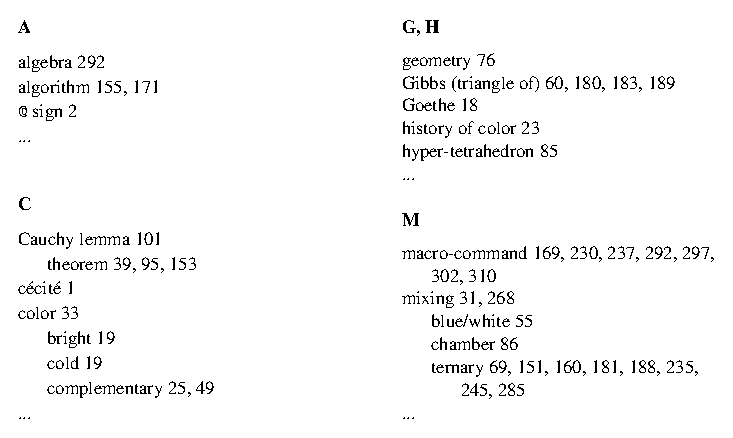
\includegraphics[width=112mm]{11.example-index.eps}
\end{center}
\vspace{4mm}
\end{fminipage}
\end{Figure}

The argument of an \cmd{index}\index{index@\cmd{index}} command contains the
mandatory level~$1$ main entry, the optional level~$2$ subentry (\emph{after}
the~``\verb+!+''~character), and the optional sort key (\emph{before}
the~``\verb+@+''~character).

Examples of level~$1$ entries are (see Figure~\ref{exemple-partiel-index}):
\begin{quote}
\index{index@\cmd{index}}
\begin{verbatim}
\index{algebra}
\index{at sign@\texttt{"@} sign}
\index{cecite@c�cit�}
\end{verbatim}
\end{quote}
\indent
If one uses method~(2) above, index entries may be written with explicit
diacritical signs (provided they use ISO-Latin~1 coding):
\begin{quote}
\index{index@\cmd{index}}
\begin{verbatim}
\index{c�cit�}
\end{verbatim}
\end{quote}

An example of level~$2$ index entry \emph{without} any specific entry for the
common word is (see Figure~\ref{exemple-partiel-index}):
\begin{quote}
\index{index@\cmd{index}}
\begin{verbatim}
\index{Cauchy!lemma}
\index{Cauchy!theorem}
\end{verbatim}
\end{quote}

An example of level~$2$ index entry \emph{with} a specific entry for the
common word is (see Figure~\ref{exemple-partiel-index}):
\begin{quote}
\index{index@\cmd{index}}
\begin{verbatim}
\index{color!}
\index{color!bright}
\index{color!cold}
\index{color!complementary}
\end{verbatim}
\end{quote}

\subsubsection{How to merge letters in the index}

If an initial letter is missing or is underrepresented, the \hermes{}
guidelines mention that this letter and an adjacent one should be merged into
one common initial (see for instance the~``G,~H''~initial in
Figure~\ref{exemple-partiel-index}).
In order to automatically produce the desired result, one should modify the
included \postawk{}\index{makeindex-post.awk@\postawk{}} filter (the use of
this filter requires the \awk{}\index{awk program@\awk{} (program)} or
\gawk{}\index{gawk program@\gawk{} (program)} program).
For instance, the following AWK~code merges the ``G''~and~``H'' initial
letters:
\begin{quote}
\begin{small}
\begin{verbatim}
/\\mkidxletter{G}/{ gsub(/{G}/,"{G, H}") ; print $0 ; next }
/\\mkidxletter{H}/{ next }
\end{verbatim}
\end{small}
\end{quote}

In order to disable this feature, it is sufficient to comment out the
relevant code lines (with the~``\verb+#+''~character).
On the other hand, the following AWK~code merges the~``I'', ``J'',~and~``K''
initial letters:
\begin{quote}
\begin{small}
\begin{verbatim}
/\\mkidxletter{I}/{ gsub(/{I}/,"{I, J, K}") ; print $0 ; next }
/\\mkidxletter{J}/{ next }
/\\mkidxletter{K}/{ next }
\end{verbatim}
\end{small}
\end{quote}

\section{Automatic typesetting procedure}

Using \bibtex{}\index{bibtex program@\bibtex{} (program)} and
\mkndx{}\index{makeindex program@\mkndx{} (program)} with \latex{} requires a
number of successive \latex{}, \bibtex{}, and \mkndx{} runs in order to get
cross-references right.
Figure~\ref{fig:Typeset} illustrates all the command lines that are required
in the case of a \emph{monograph} (we assume that the master \latex{} source
file is \file{\meta{master}.tex}).

\begin{Figure}[!htbp]{%
The typesetting procedure\label{fig:Typeset}}
\begin{fminipage}
\vspace{6pt}
\HS{}\texttt{latex~\meta{master}.tex}\\
\HS{}\texttt{bibtex~\meta{master}.aux}\\
\HS{}\texttt{latex~\meta{master}.tex}\\
\HS{}\texttt{latex~\meta{master}.tex}\\
\HS{}\texttt{makeindex~-c~-l~-s~ouvrage-hermes.ist~\meta{master}.idx}\\
\HS{}\texttt{latex~\meta{master}.tex}\\
\HS{}\texttt{latex~\meta{master}.tex}\\
\HS{}\texttt{dvips~-t~a4~\meta{master}.dvi}
\vspace{6pt}
\end{fminipage}
\index{bibtex program@\bibtex{} (program)}
\index{makeindex program@\mkndx{} (program)}
\index{ouvrage-hermes.ist@\istyle{ouvrage-hermes}}
\index{dvips driver@\dvips{} (driver)}
\end{Figure}

In the case of an \emph{edited collection}, the \bibtex{} command line of
Figure~\ref{fig:Typeset} shall be replaced by a \bibtex{} run on each chapter
file name (the \bibtex{} program shall be run once on each chapter that
possesses a bibliography section).

The \oh{} package includes\index{Makefile script@\Makefile{} (script)} a
generic \Makefile{} script that should be configured in order to drive the
\make{}\index{make program@\make{} (program)} program (this program is
available under Unix, GNU/Linux, *BSD, Mac OS~X, and Microsoft Windows/Cygwin
platforms).
The \Makefile{} script automates the whole typesetting procedure.


%%% Local Variables: 
%%% mode: latex
%%% TeX-master: "users-guide.ltx"
%%% End: 
